\section{Additional Figures and Tables}
\label{sec:si-figures}

\clearpage

% ================================
% Active Space representability 
% ================================
% Graph of the errors vs projection deficit
\begin{figure}[htbp]
    \centering
    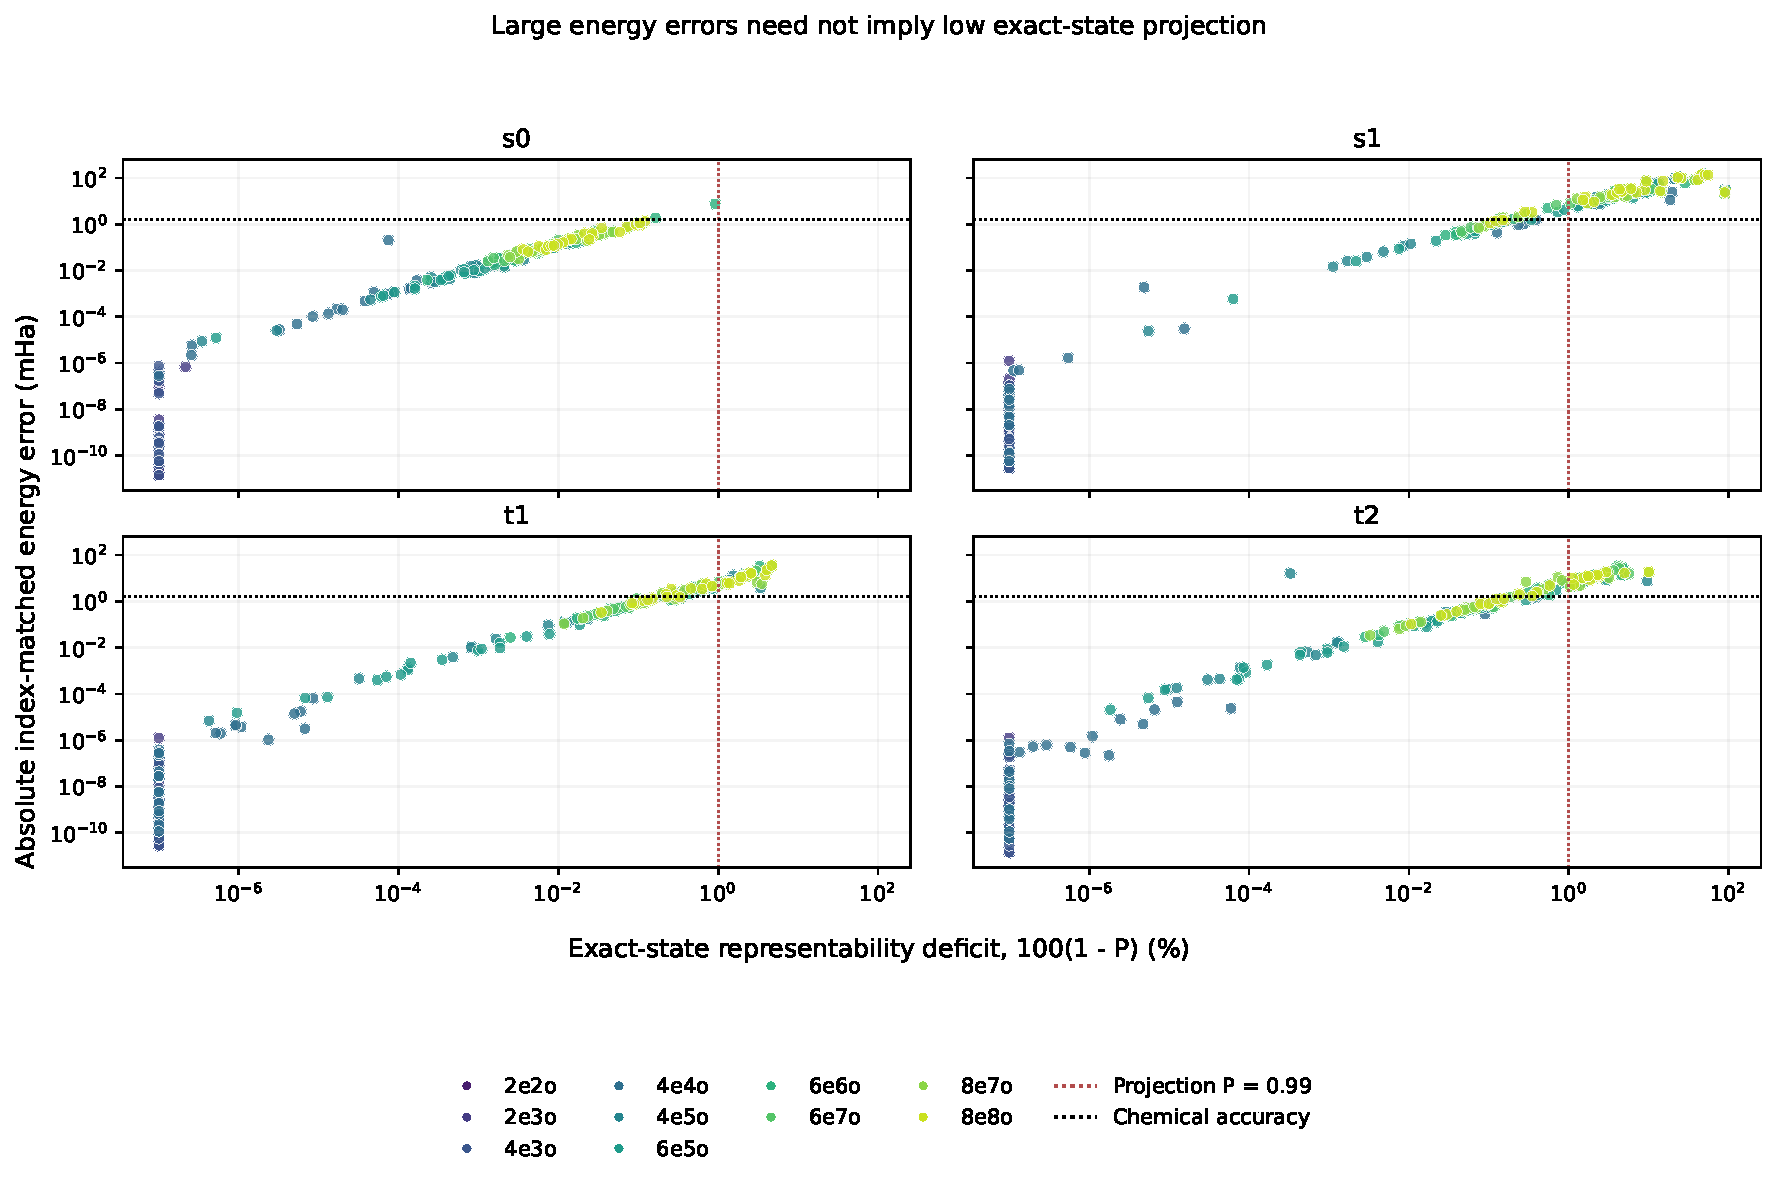
\includegraphics[width=\linewidth]{figures/active_space_representability/uccsd_error_vs_projection_deficit.pdf}
    \caption{Absolute UCCSD QSE energy error as a function of the missing projection of the exact state outside the QSE subspace. Results are shown for the low-lying singlet and triplet states across the molecular benchmark.}
    \label{fig:si-error-vs-projection-deficit}
\end{figure}

% Graph of double excitation weight CASCI singlet and triplet states 
\begin{figure}[htbp]
    \centering
    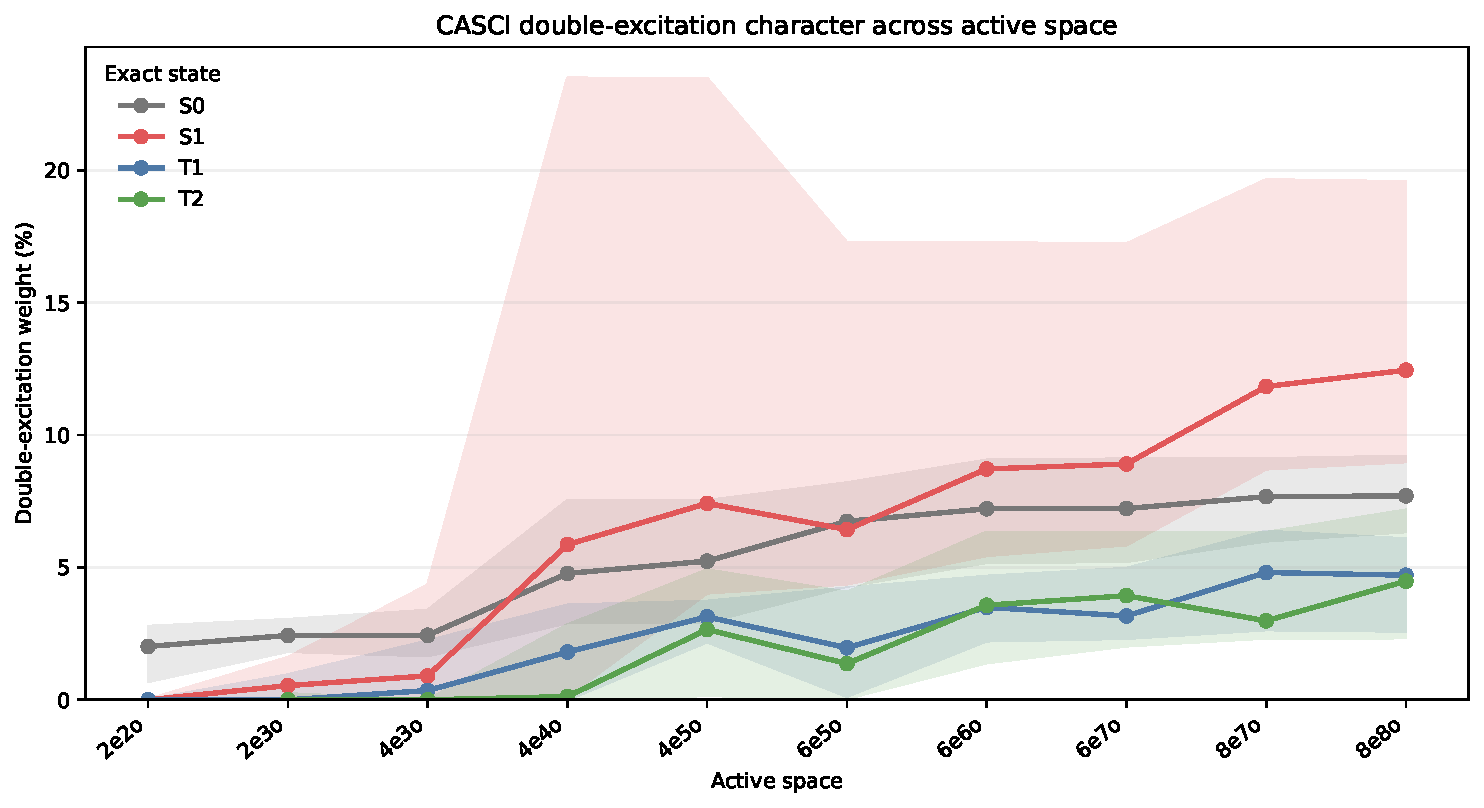
\includegraphics[width=\linewidth]{figures/active_space_representability/casci_doubles_weight/low_state_double_excitation_weight_scaling.pdf}
    \caption{Double-excitation weight of the exact CASCI low-lying singlet and triplet states across active spaces. Solid lines show the median double-excitation weight for the $S_1$, $T_1$, and $T_2$ states across the molecular benchmark; shaded regions show the corresponding distribution ranges.}
    \label{fig:si-casci-double-excitation-weight}
\end{figure}

% Graph of the best overlap root match for Q1
\begin{figure}[htbp]
    \centering
    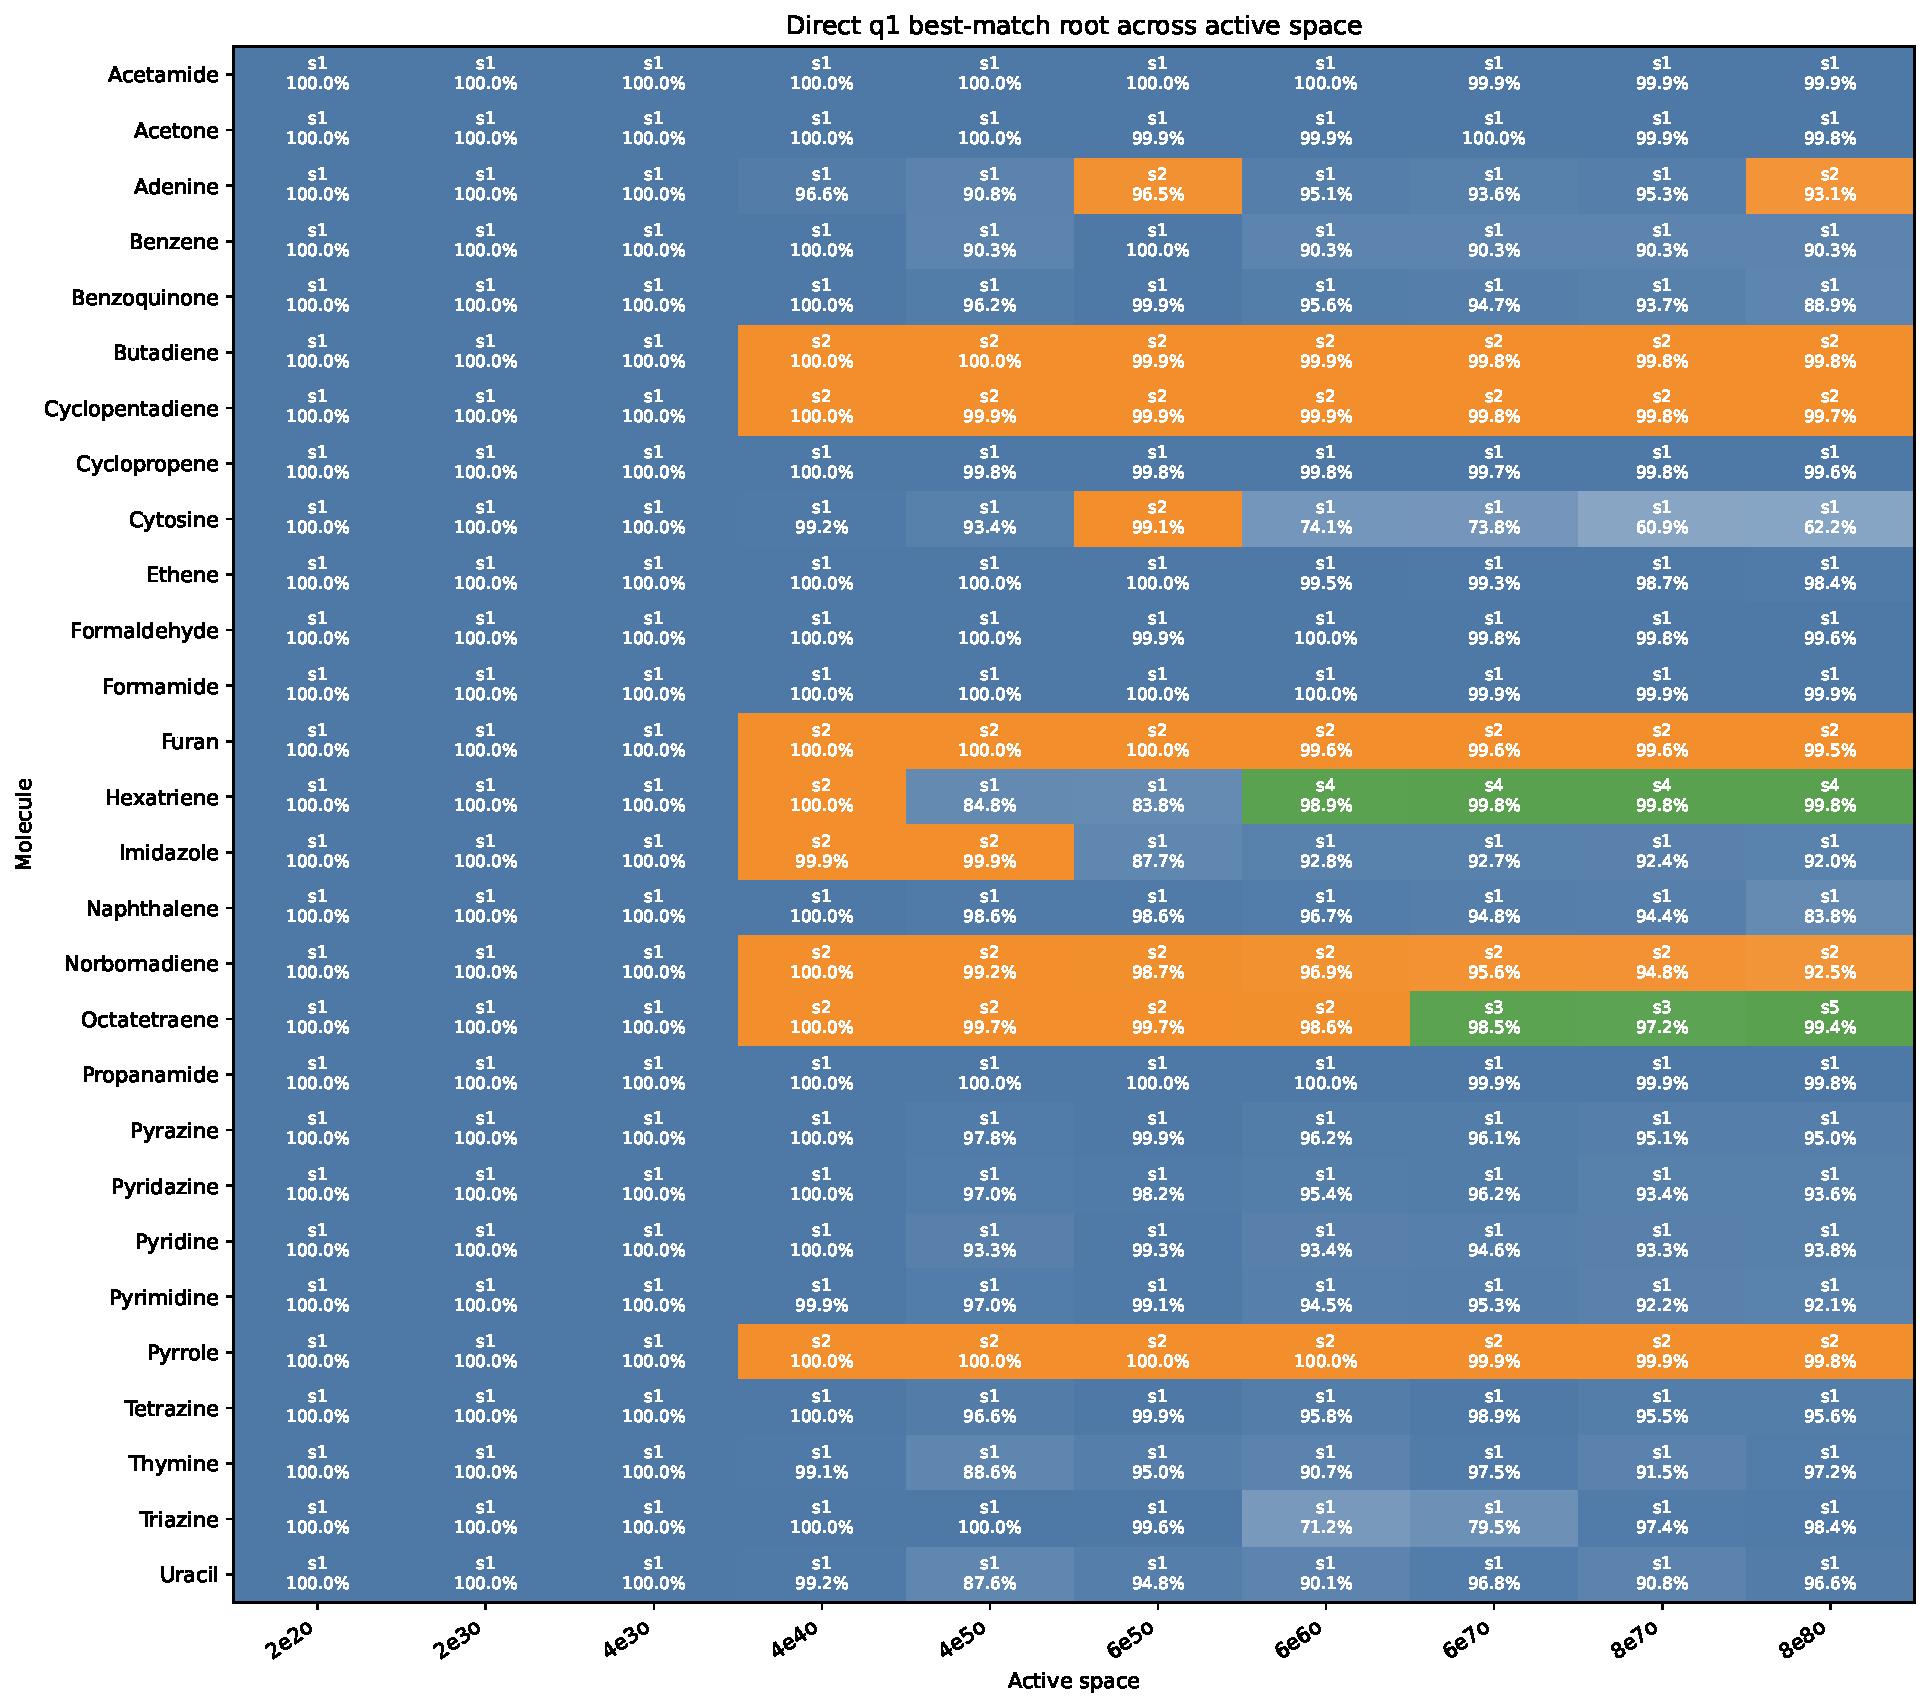
\includegraphics[width=\linewidth]{figures/active_space_representability/uccsd_q1_best_root_transition_map.pdf}
    \caption{Best-overlap root assignment for the UCCSD QSE calculation across active spaces. The map shows how the exact target roots are matched to the QSE roots under maximum-overlap matching.}
    \label{fig:si-q1-best-root-transition-map}
\end{figure}

% ================================
% Dimension analysis
% ================================

\begin{figure}[htbp]
    \centering
    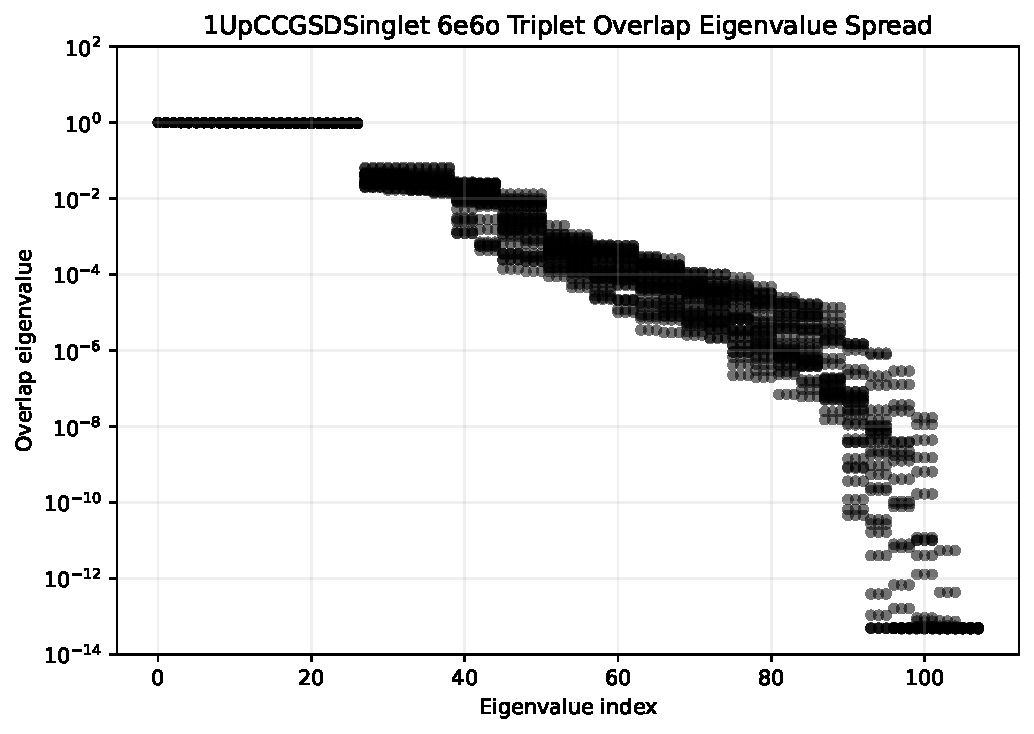
\includegraphics[width=\linewidth]{figures/dimension_analysis/overlap_eigenvalue_spread/1upccgsdsinglet_triplet_6e6o.pdf}
    \caption{1UpCCGSDSinglet overlap-eigenvalue spread for the $6e6o$ singlet and triplet sectors.}
    \label{fig:si-1up-triplet-eigenvalues}
\end{figure}

\begin{figure}[htbp]
    \centering
    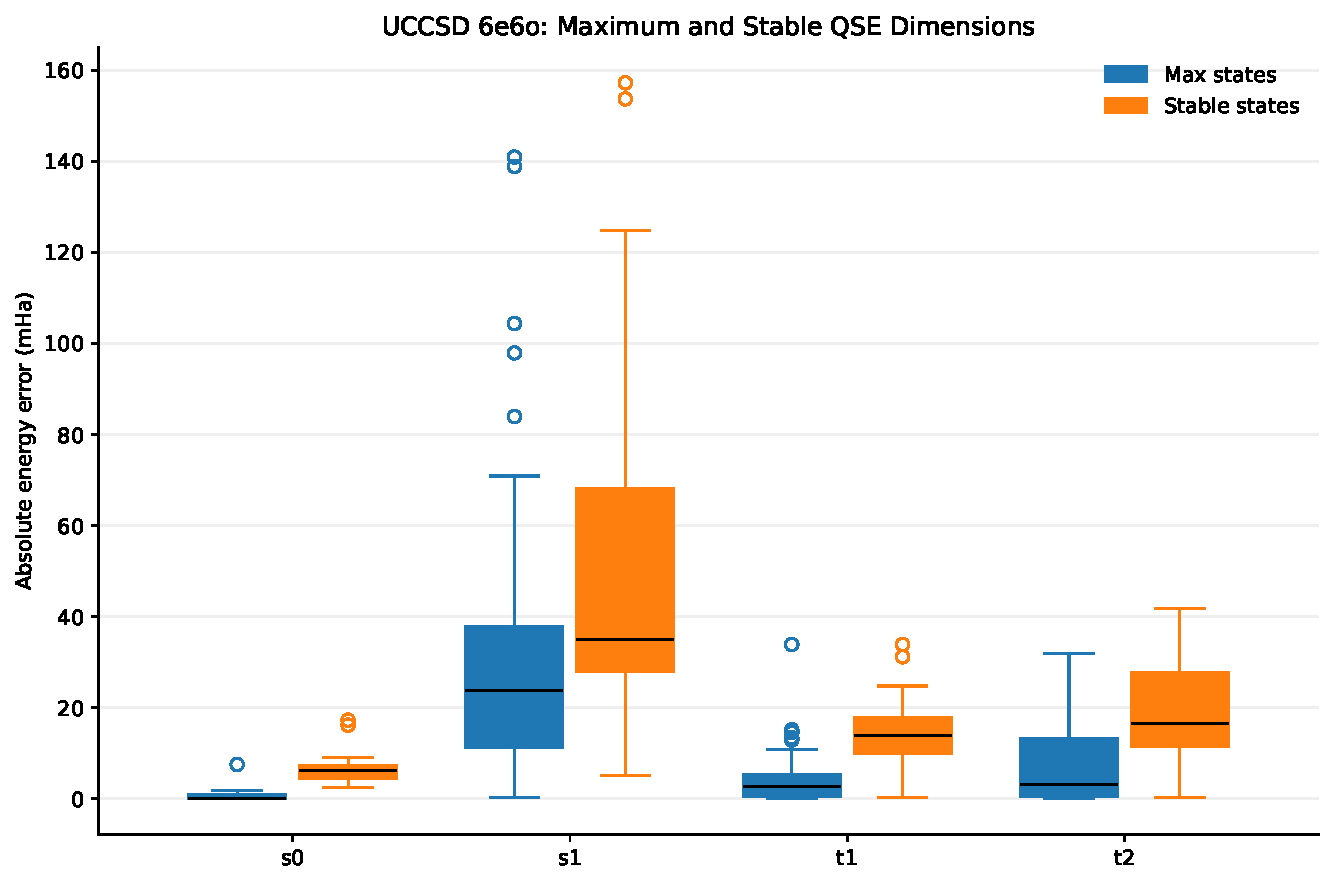
\includegraphics[width=\linewidth]{figures/dimension_analysis/max_stable_error_distribution_6e6o.pdf}
    \caption{Molecule-level index-matched errors for the low-lying $s0$, $s1$, $t1$, and $t2$ roots in the UCCSD $6e6o$ active space, comparing the maximum retained QSE dimension with the overlap-stable dimension.}
    \label{fig:si-max-stable-error-distribution}
\end{figure}

% ================================
% Shots
% ================================
\begin{figure}[htbp]
    \centering
    
\includegraphics[width=\linewidth]{figures/shots/eigenvalue_lifting/uccsd_6e6o.pdf}
    \caption{Finite-shot lifting of UCCSD overlap eigenvalues in the $6e6o$ active space.}
    \label{fig:si-eigenvalue-lifting}
\end{figure}


% ================================
% Scaling future work
% ================================
\begin{figure}[htbp]
    \centering
    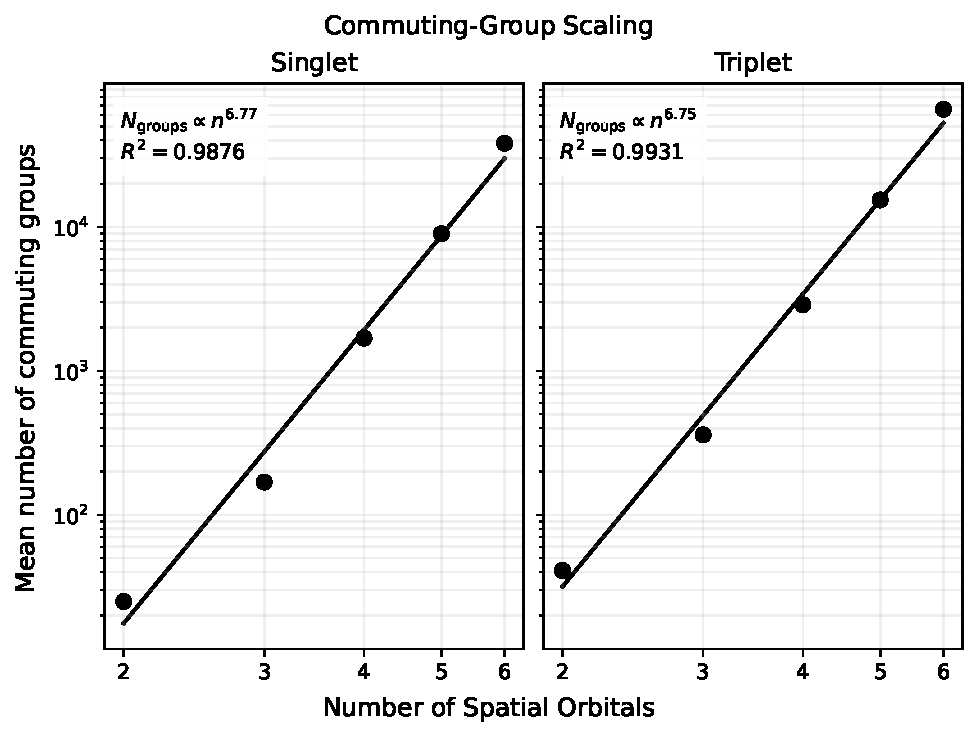
\includegraphics[width=\linewidth]{figures/scaling_future_work/commuting_group_scaling.pdf}
    \caption{Scaling of the number of commuting measurement groups with active-space size for the projected QSE matrices.}
    \label{fig:si-commuting-group-scaling}
\end{figure}

\begin{figure}[htbp]
    \centering
    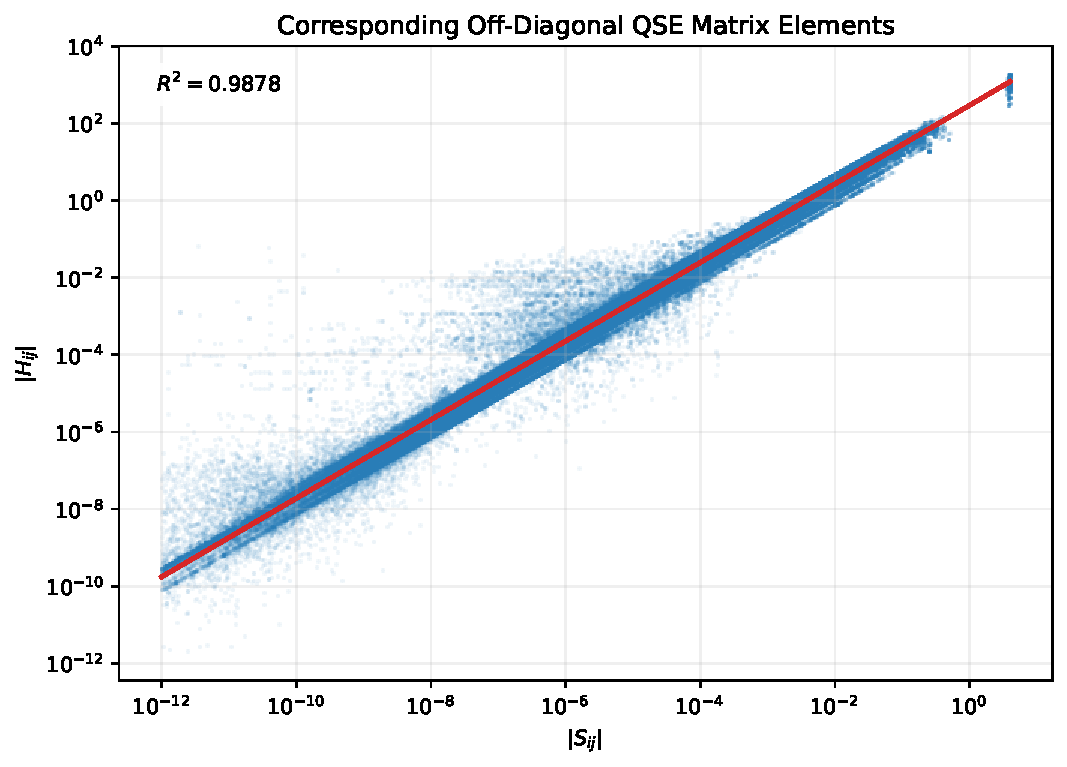
\includegraphics[width=\linewidth]{figures/scaling_future_work/matrix_heatmaps/uccsd_h_s_element_regression.pdf}
    \caption{Correlation between projected Hamiltonian and overlap matrix elements for the UCCSD QSE calculation in the $6e6o$ active space.}
    \label{fig:si-h-s-element-correlation}
\end{figure}

\begin{figure}[htbp]
    \centering
    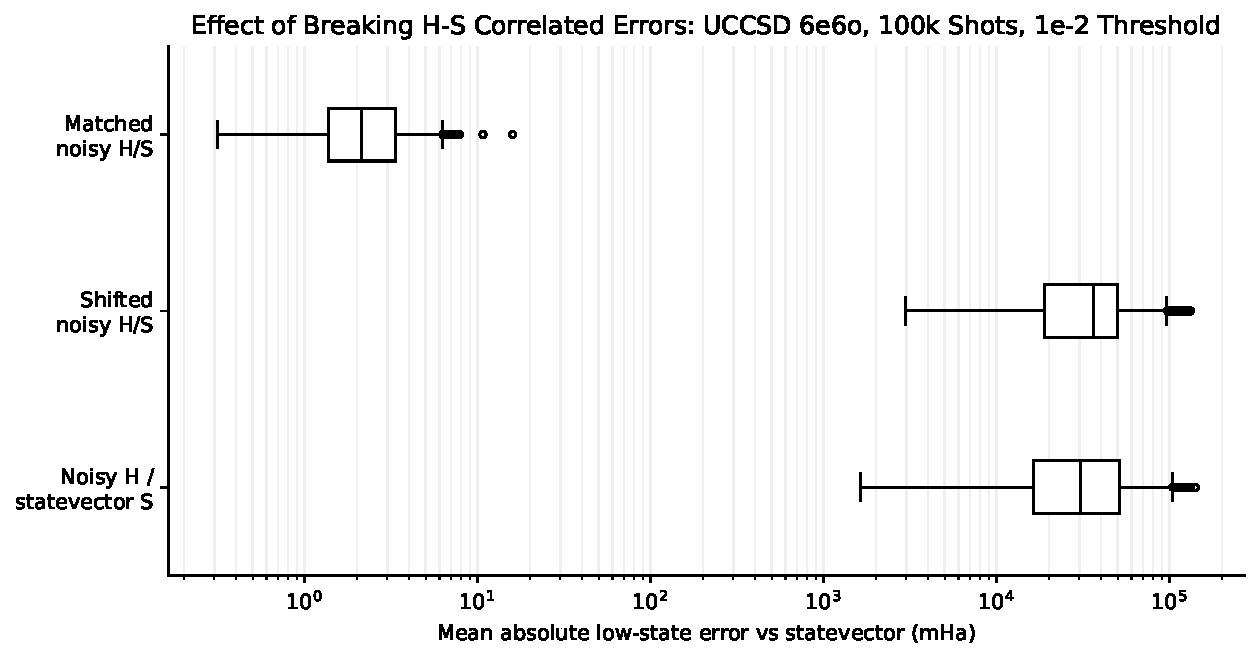
\includegraphics[width=\linewidth]{figures/scaling_future_work/breaking_hs_correlated_errors.pdf}
    \caption{Effect of breaking the correlation between projected Hamiltonian and overlap-matrix errors on the reconstructed QSE spectrum.}
    \label{fig:si-breaking-h-s-correlated-errors}
\end{figure}

\begin{figure}[htbp]
    \centering
    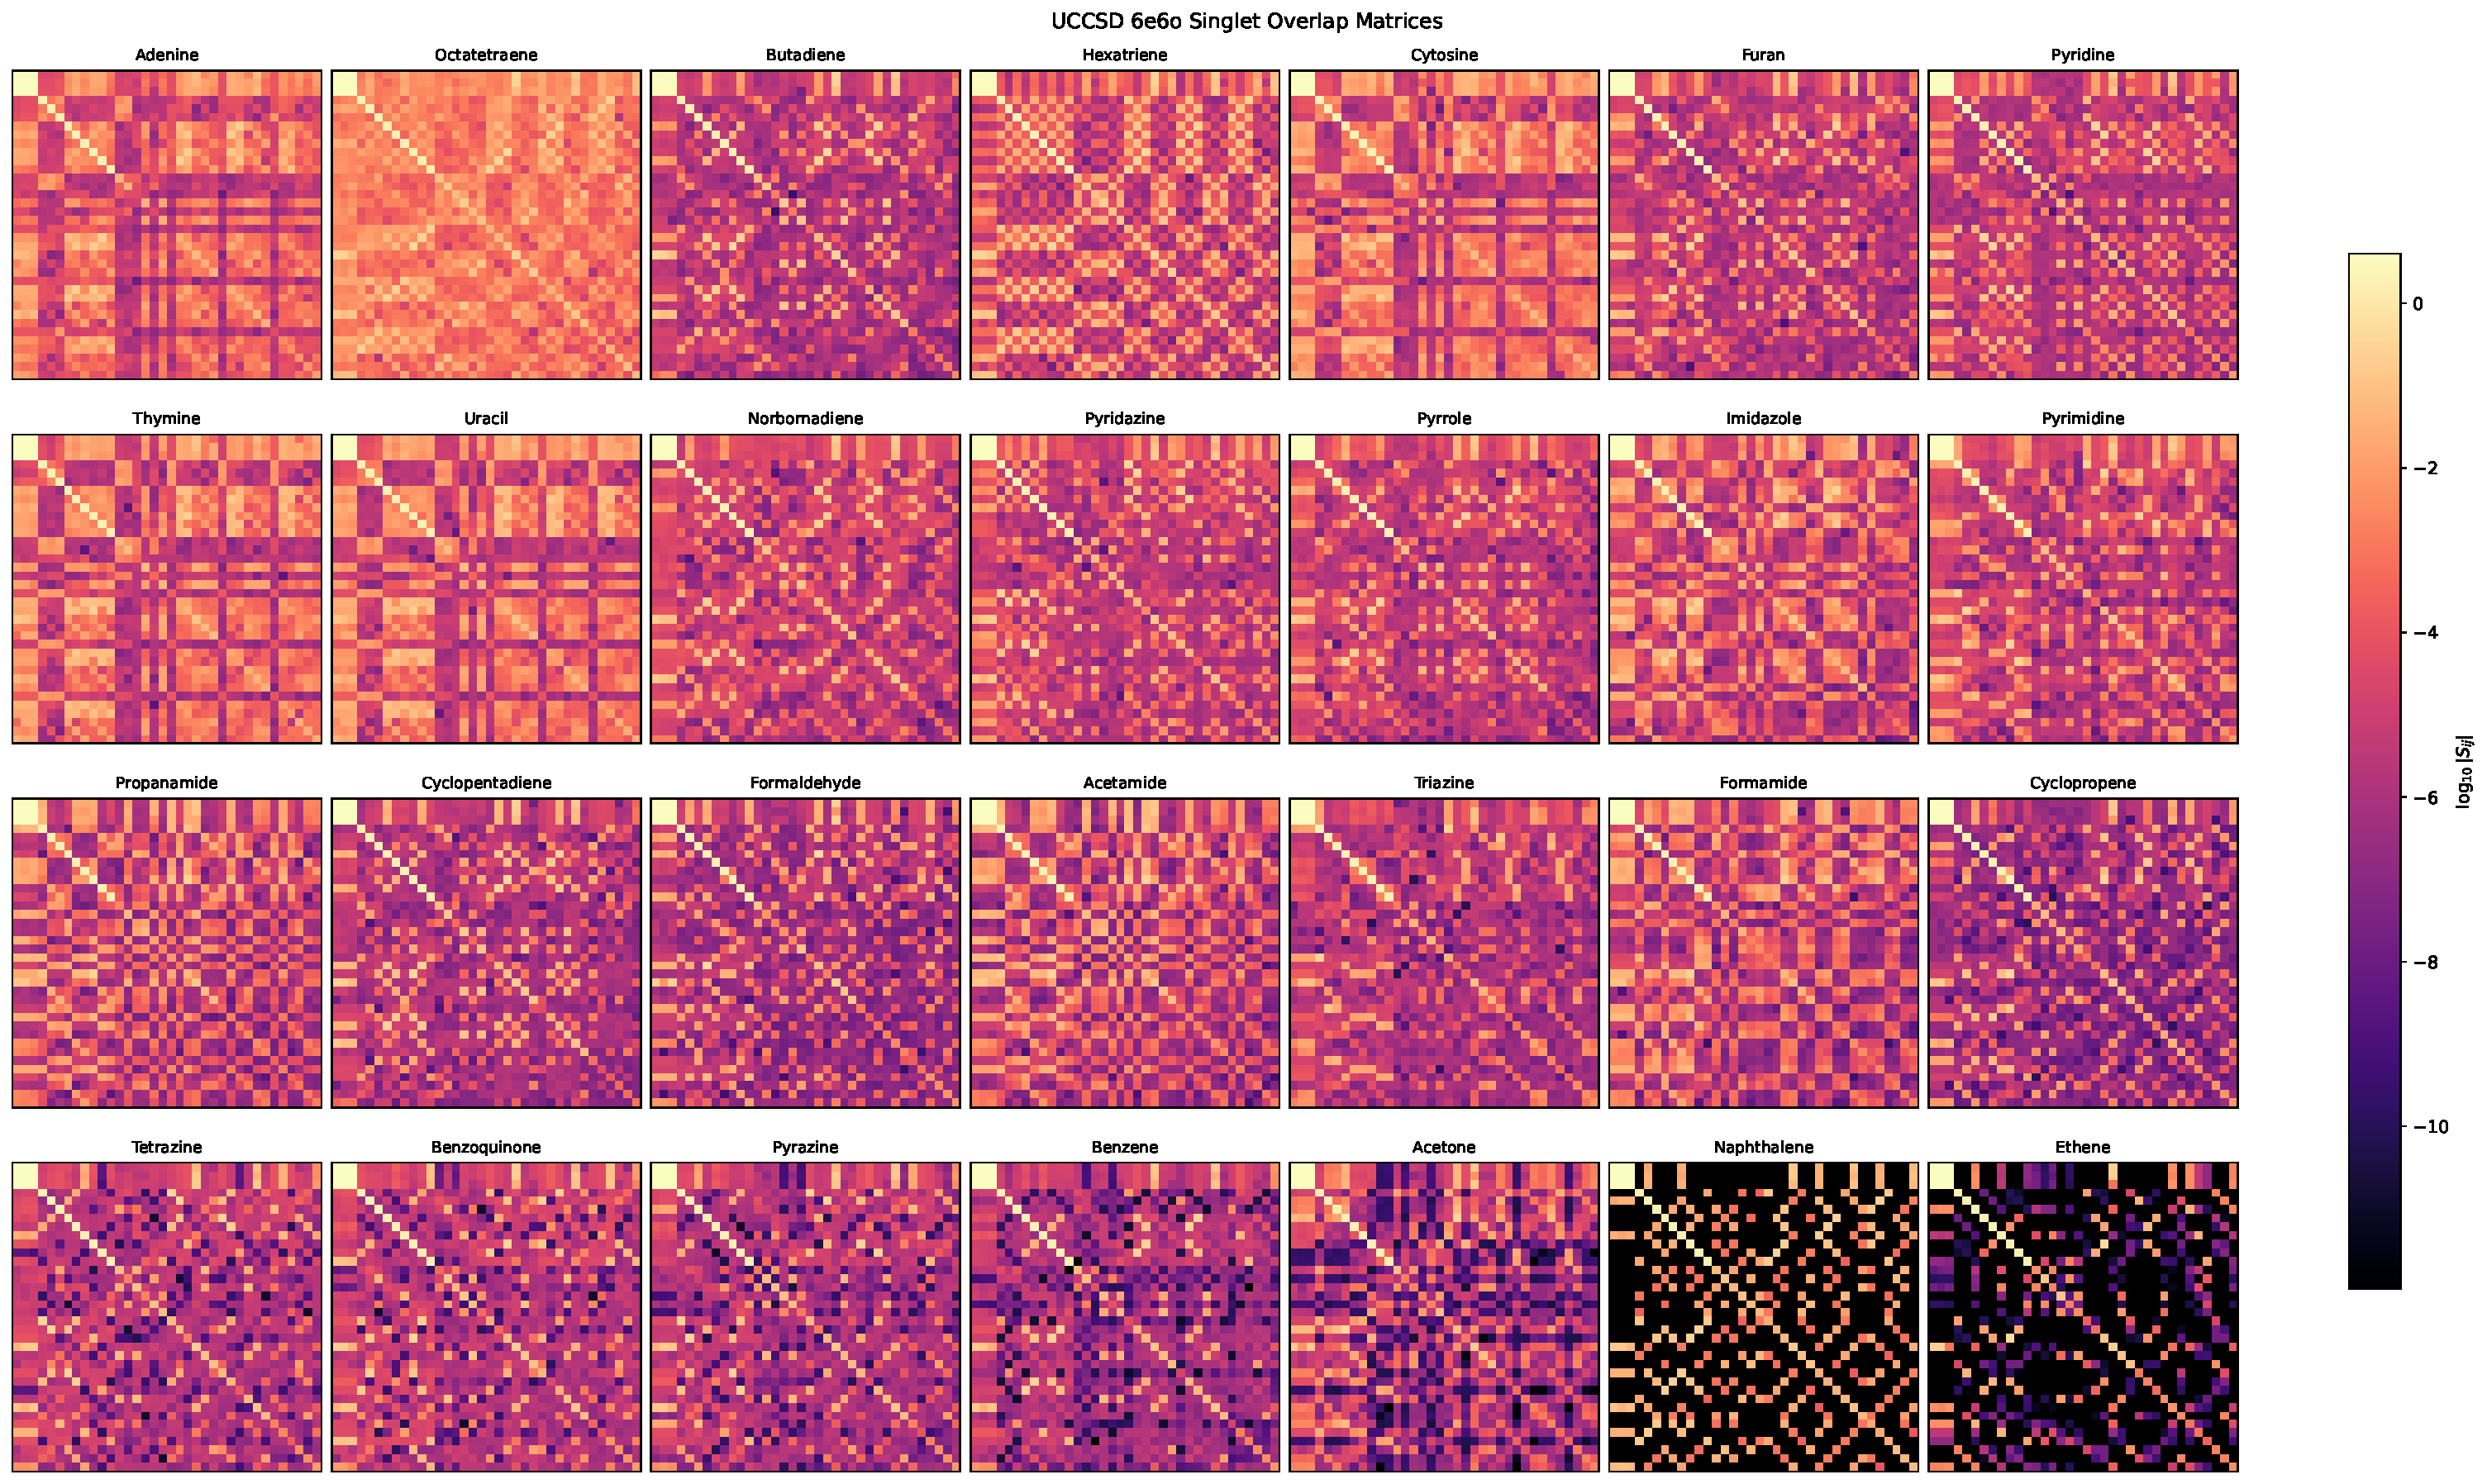
\includegraphics[width=\linewidth]{figures/scaling_future_work/matrix_heatmaps/uccsd_6e6o_singlet_overlap.pdf}
    \caption{Full 28-molecule singlet overlap heatmaps comparing statevector and shot-based results.}
    \label{fig:si-full-singlet-heatmaps}
\end{figure}

\begin{figure}[htbp]
    \centering
    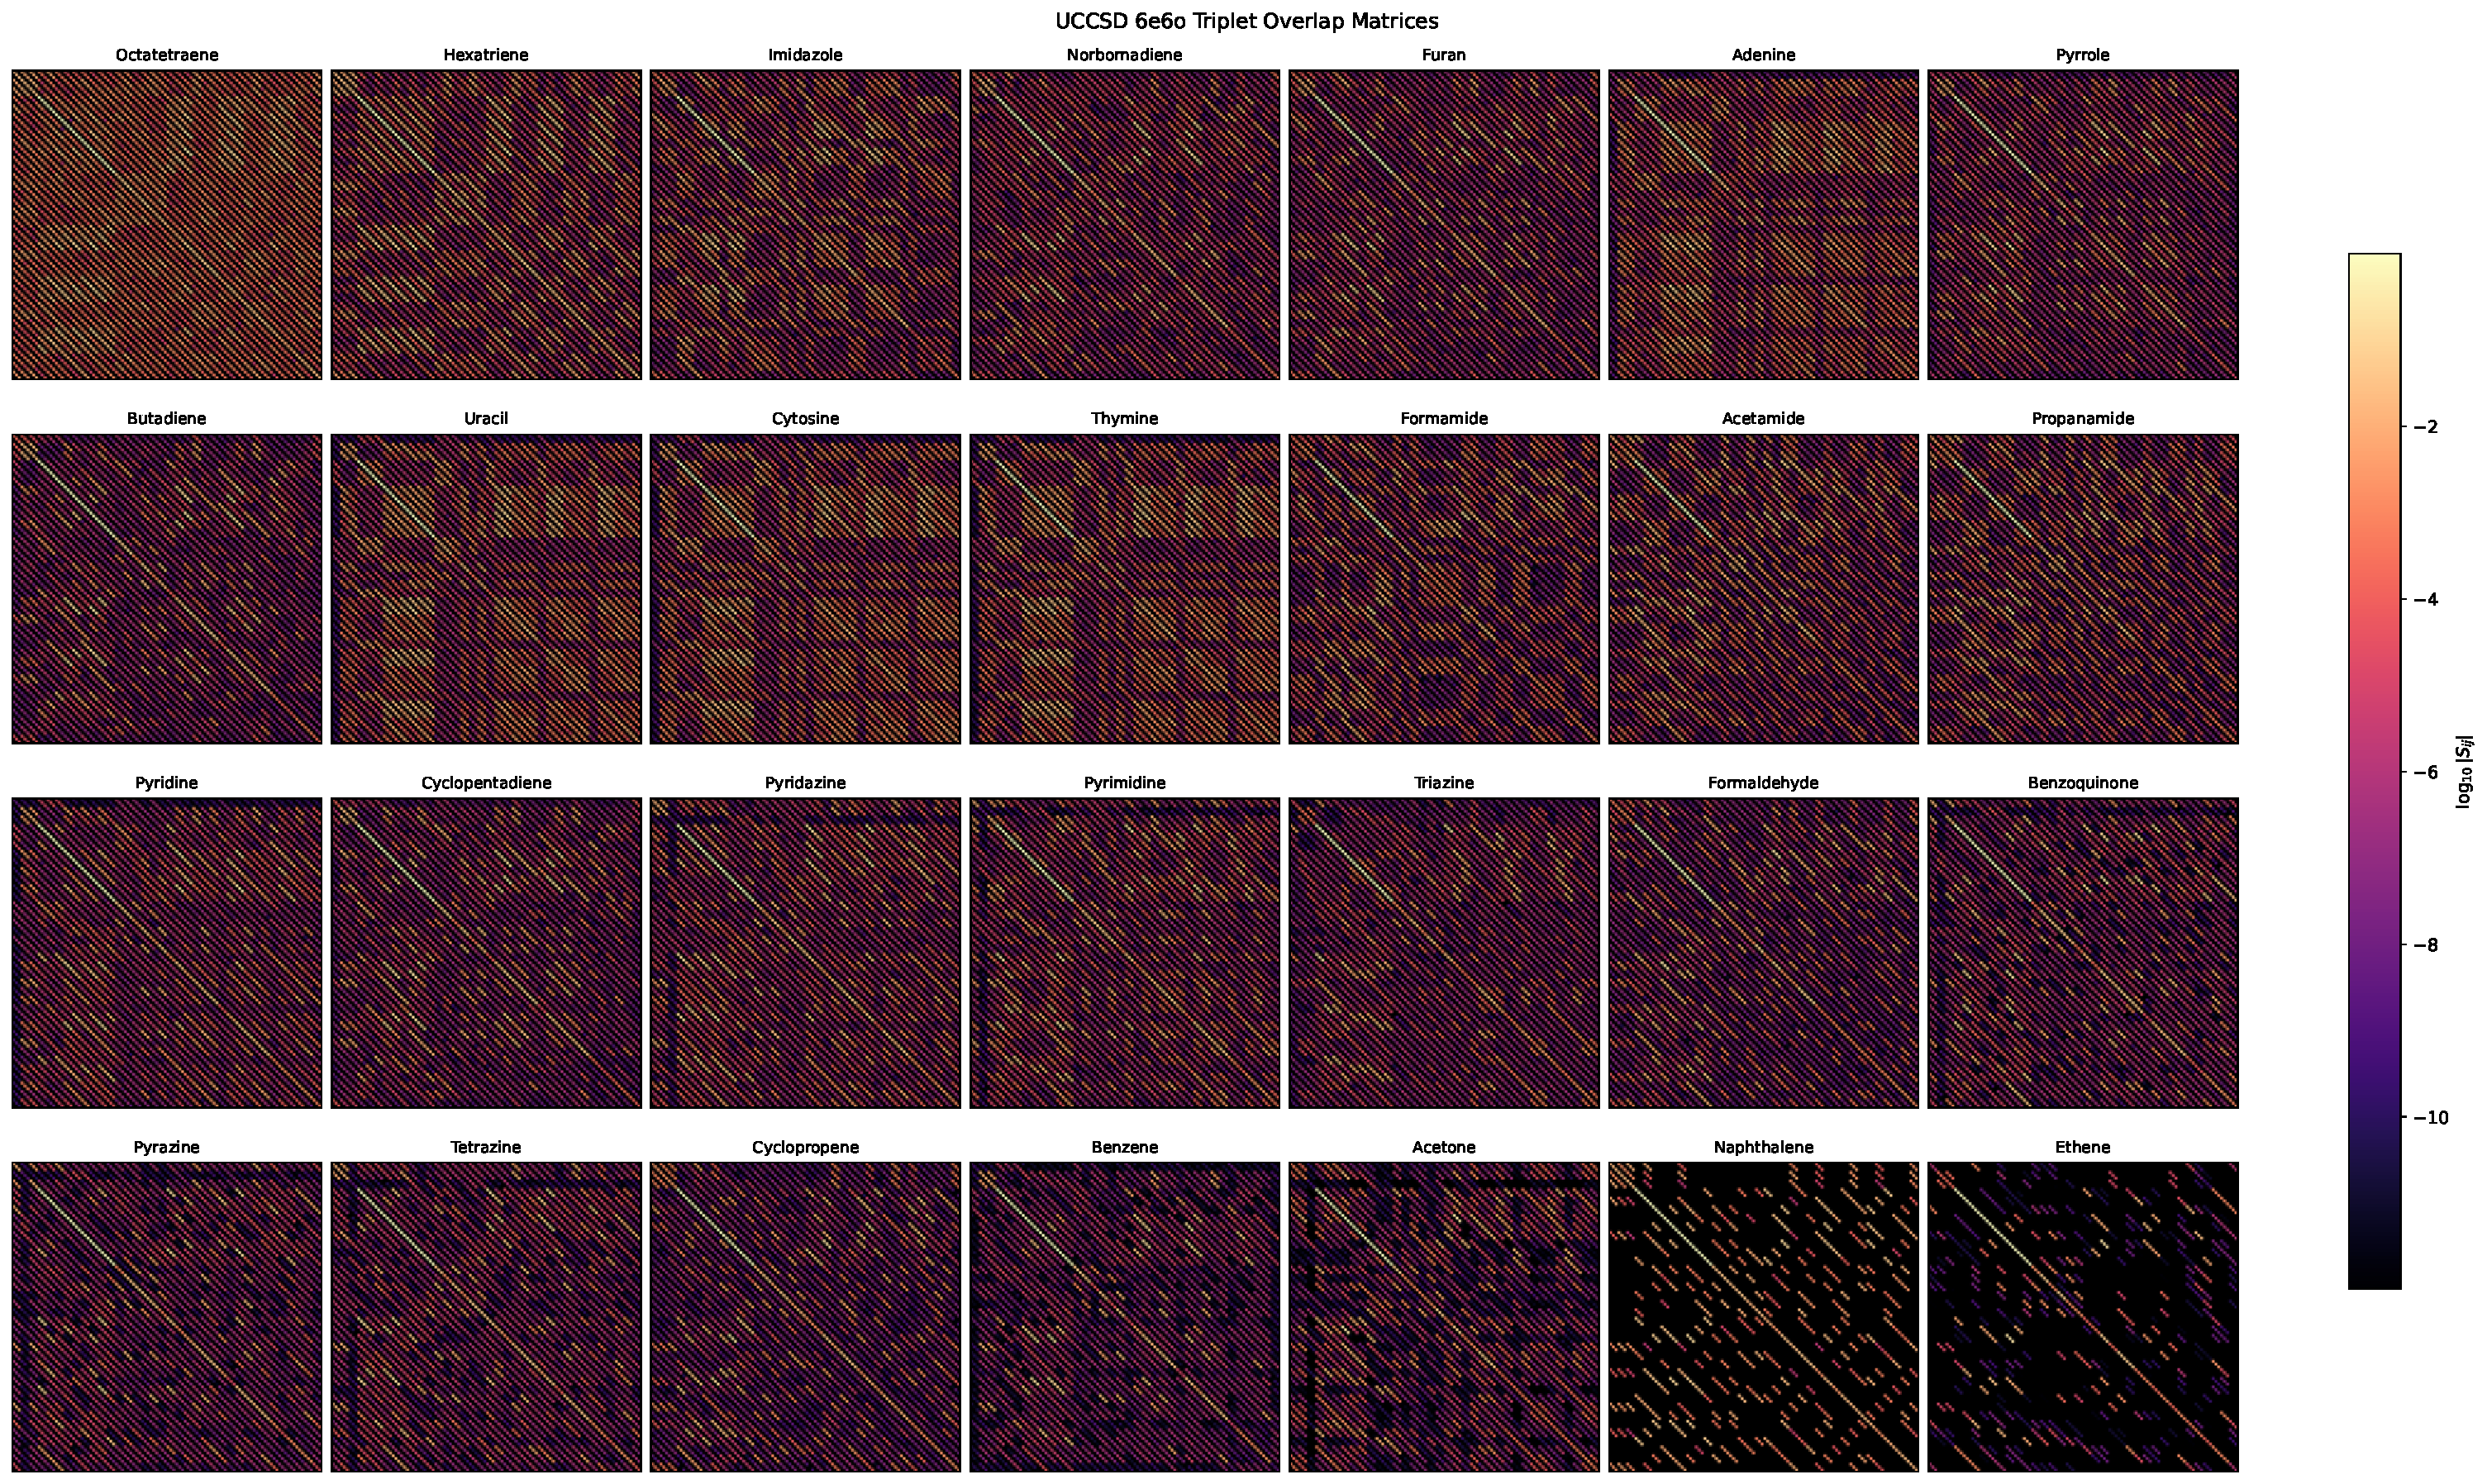
\includegraphics[width=\linewidth]{figures/scaling_future_work/matrix_heatmaps/uccsd_6e6o_triplet_overlap.pdf}
    \caption{Full 28-molecule triplet overlap heatmaps comparing statevector and shot-based results.}
    \label{fig:si-full-triplet-heatmaps}
\end{figure}
